\documentclass[12pt,a4paper]{article}

\usepackage[utf8]{inputenc}
\usepackage[T1]{fontenc}
\usepackage[portuguese]{babel}

\usepackage{listings}
\usepackage{xcolor}
\usepackage{amsmath}
\usepackage{amssymb}
\usepackage{amsfonts}
\usepackage{graphicx}

\lstset{
    basicstyle=\ttfamily\small,
    keywordstyle=\color{blue}\bfseries, 
    commentstyle=\color{green!70!black},
    stringstyle=\color{red}, 
    numbers=left, 
    numberstyle=\tiny\color{gray}, 
    frame=single, 
    breaklines=true, 
    showstringspaces=false 
}

\usepackage[margin=2.5cm]{geometry}

\begin{document}

\begin{center}
    {\LARGE MC521 - Relatório II} \\ [2,5em]
    {\large Júlio da Silva Telles} \\ [1,0em]
    {\large 12 de Julho de 2026} \\ [1,5em]
\end{center}

\vspace{1cm} 

\section{D - Asya and Kittens (CodeForces - 1131F)}

O problema D descreve uma situação em que temos $n$ gaiolas numeradas de $1-n$ lado a lado cada uma contendo um gato. Em um certo momento pares de 
gatos em celas adjacentes podem formar pares, então remove-se a divisão entre suas gaiolas para que possam brincar, até que todos os gatos estejam
na mesma gailoa. Dado apenas a ordem em que as uniões de gaiolas foram estabelecidas o problema pede a ordem inicial em que as gaiolas estevam, antes
da junção dos pares. A imagem abaixo contem um dos varios possiveis arranjos iniciais de gaiolas para o seguinte caso teste: $ {(1, 4),(2, 5),(3, 1), (4, 5)}$ 

\begin{figure}[!htb]
    \centering
    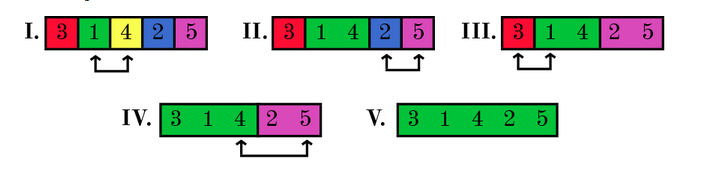
\includegraphics[width=0.8\textwidth]{cells.png}
    \caption{Legenda descritiva da sua imagem.}
    \label{fig:minha_imagem}
\end{figure}

\subsection{Solução}

Vamos utilizar um algorimtmo de DSU para resolver esse problema. O algoritmo realiza a união de conjuntos dinâmicos de forma eficiente e registra o histórico dessas conexões. O objetivo principal é imprimir a sequência unificada de elementos na ordem inversa: partindo da \textbf{folha} (fim da fusão) até a \textbf{raiz} (início da fusão). Para isso, gerenciam-se duas estruturas de dados simultâneas: uma árvore para os conjuntos e uma lista encadeada para a ordenação.
\begin{itemize}
    \item {Inicialização}: Cada elemento começa isolado em seu próprio conjunto, sendo simultaneamente a \textbf{cabeça} (início) e a \textbf{cauda} (fim) de sua respectiva lista encadeada.
    \item Operação de União (\texttt{unionSet}): Ao unir dois elementos, o algoritmo executa dois passos independentes:
    \begin{itemize}
        \item \textbf{Otimização do DSU (Árvore):} Utiliza a heurística de \textit{rank}, conectando a raiz da árvore menor à raiz da árvore maior. Isso garante que a altura da árvore permaneça mínima, mantendo a complexidade de busca quase constante $\mathcal{O}(\alpha(N))$.
        \item \textbf{Encadeamento das Listas (Ordem):} Conecta o fim (cauda) da lista do primeiro conjunto ao início (cabeça) da lista do segundo conjunto. A cauda do conjunto resultante é atualizada para ser a cauda do segundo grupo.
    \end{itemize}

\end{itemize}

Após todas as uniões e retornamos a ordem especifica de impressão guardada na lista encadeada.

\end{document}  